% ### Uses XeLaTeX ### %
% ### Needs beamer-master ### %
\documentclass[aspectratio=169]{beamer} %. Aspect Ratio 16:9
\usetheme{AI2} % beamerthemeSprace.sty
% DATA FOR FOOTER
\date{2020}
\title{Workflows de trabalho utilizando git}
\author{}
\institute{Advanced Institute for Artificial Intelligence (AI2)}
\usepackage{color}
\usepackage{xcolor}
\usepackage{listings}
\usepackage[T1]{fontenc}
\usepackage[utf8]{inputenc}
%--------------------------------------

%Portuguese-specific commands
%--------------------------------------
\usepackage[portuguese]{babel}

\begin{document}
% ####################################
% FIRST SLIDE 						:: \SliTit{This is the Title of the Talk}{A. B. Name}{Sprace}
% SUB-TITLE SLIDE 					:: \SliSubTit{<title>}{<explanation}
% SUB-SUB-TITLE SLIDE				:: \SliSubSubTit{<title>}{<explanation}
% SLIDE WITH TITLE 					:: \SliT{Title}{Content}
% SLIDE NO TITLE 						:: \Sli{Content} 
% SLIDE DOUBLE COLUMN WITH TITLE 	:: \SliDT{Title}{First Column}{Second Column}
% SLIDE DOUBLE COLUMN NO TITLE 		:: \SliD{First Column}{Second Column}
% SLIDE ADVANCED WITH TITLE 			:: \SliAdvT{Title}{Content}
% SLIDE ADVANCED NO TITLE 			:: \SliAdv{Content}
% SLIDE ADVANCED DOUBLE WITH TITLE 	:: \SliAdvDT{Title}{First Column}{Second Column}
% SLIDE ADVANCED DOUBLE NO TITLE 	:: \SliAdvD{First Column}{Second Column}
% SLIDE BLACK						:: \Black{ <Content> }
% SLIDE WHITE						:: \White{ <Content> }
% ITEMIZATION 						:: \begin{itemize}  \iOn{First} \iTw {Second} \iTh{Third} \end{itemize}
% COMMENT TEXT				 		:: \note{<comment>}
% SECTION 							:: \secx{Section} | \secxx{Sub-Section}
% BOLD SPRACE COLOR				:: \bfs{<text>}
% TABLE OF CONTENT					:: \tocitem{<title>}{<content>}
% LEFT ALIGN EQUATION				:: \begin{flalign*}  & <equation> &   \end{flalign*}
% CENTER ALIGN EQUATION	S			:: \begin{gather*} <equations>  \end{gather*}
% SLASH								:: \slashed{<>}
% BAR								:: \barr{<letter>} instead of \bar{<letter>}
% THEREFORE						:: use \portanto (larger and bold}
% 2 or 3 MATH SYMBOLS				:: \overset{<up>}{<down>} &  \underset{<below>}{\overset{<above>}{<middle>}}  
% INSERT TEXT IN FORMULA			:: \ins{<text>}
% EXERCISE							:: \exe{<exercise #>}{<exercise text>}
% SUGGESTED READING BOX			:: \sug{<references>}
% CITATION							:: \cittex{<citation>}
% CITATION DOUBLE COLUMN 			:: \cittexD{<citation>}
% TEXT POSITION						:: \texpos{<Xcm>}{<Ycm>}{<text>} origin = center of slide : x right | y down
% REFERENCE AT BOTTOM  S/D SLIDE		:: \refbotS{<reference>} \refbotD{<reference>}
% HIDDEN SLIDE						:: \hid
% COLOR BOX 						:: \blu{blue} + \red{rec} + \yel{yellow} + \gre{green} + \bege{beige}
% FRAME 							:: \fra{sprace} \frab{blue} \frar{red} + \fray{yellow} + \frag{green}		
% FIGURE 							:: \img{X}{Y}{<scale>}{Figure.png} 
% FIGURE							:: \includegraphics[scale=<scale>]{Figures/.png}
% FIGURE DOUBLE SLIDE NO TITLE		::  \img{-4}{0.5}{<scale>}{Figure.png} % Image 1st half
%									::  \img{4}{0.5}{<scale>}{Figure.png} % Image 2nd half
% FIGURE DOUBLE SLIDE WITH TITLE		::  \img{-4}{0}{<scale>}{Figure.png} % Image 1st half
%									::  \img{4}{0}{<scale>}{Figure.png} % Image 2nd half
% INCLUDING SWF (Flash)				:: \usepackage{media9} and \includemedia >> USE ACROBAT <<
%%%%%%%%%%%%%%%%%%%%%%%%%%%%%%%%%%%%%%%%%%%%%%%%%%
% ###############################################################################
% FIRST SLIDE
\SliTit{Workflows de trabalho utilizando git}{Advanced Institute for Artificial Intelligence -- AI2}{https://advancedinstitute.ai}
%%%%%%%%%%%%%%%%%%%%%%%%%%%%%%%%%%%%%%%%%%%%%%%%%%
% ###############################################################################
% SLIDE SUB-TITLE
\SliSubTit{}{Exemplos retirados do tutorial da
\href{https://www.atlassian.com/br/git/tutorials/comparing-workflows}{Atlassian}}{}
%%%%%%%%%%%%%%%%%%%%%%%%%%%%%%%%%%%%%%%%%%%%%%%%%%
% ###############################################################################
%\SliSubSubTit{Sub-Sub-Title}{Description}
 %%%%%%%%%%%%%%%%%%%%%%%%%%%%%%%%%%%%%%%%%%%%%%%%%%
% ###############################################################################
% SLIDE WITH TITLE

\SliT{Fluxo de trabalho do Git}{
    \cittex{Receita ou recomendação sobre como usar o Git para realizar o 
    trabalho de maneira consistente e produtiva}

\begin{itemize}

      \iOn{Reforçam para os usuários a necessidade de utilizar o Git de modo
        eficiente e consistente}

      \iOn{Git possui muita flexibilidade. Portanto, não há um processo
        padronizado para colaboração}

      \iOn{É importante que a equipe esteja de acordo com como o fluxo de
        de trabalho proposto}

\end{itemize}
}

\SliT{Fluxo de trabalho do Git}{
\begin{itemize}

    \iOn{É muito importante considerar a cultura da equipe}

    \iOn{Algumas coisas a considerar ao avaliar um fluxo de trabalho do Git
        são:}

    \begin{itemize}

        \iTw{\textbf{Este fluxo de trabalho está de acordo com o tamanho da
            equipe?}}

        \iTw{\textbf{É fácil desfazer erros com este fluxo de trabalho?}}

        \iTw{\textbf{Este fluxo de trabalho impõe alguma sobrecarga à equipe?}}

    \end{itemize}
\end{itemize}
}

\SliSubTit{Workflow Centralizado}{}

\SliT{Fluxo de trabalho centralizado}{
\begin{itemize}

    \iOn{Boa alternativa para equipes em transição do SVN}

    \iOn{Usa um repositório central que serve como único ponto de entrada para
        todas as mudanças no projeto}

\end{itemize}
\begin{center}
    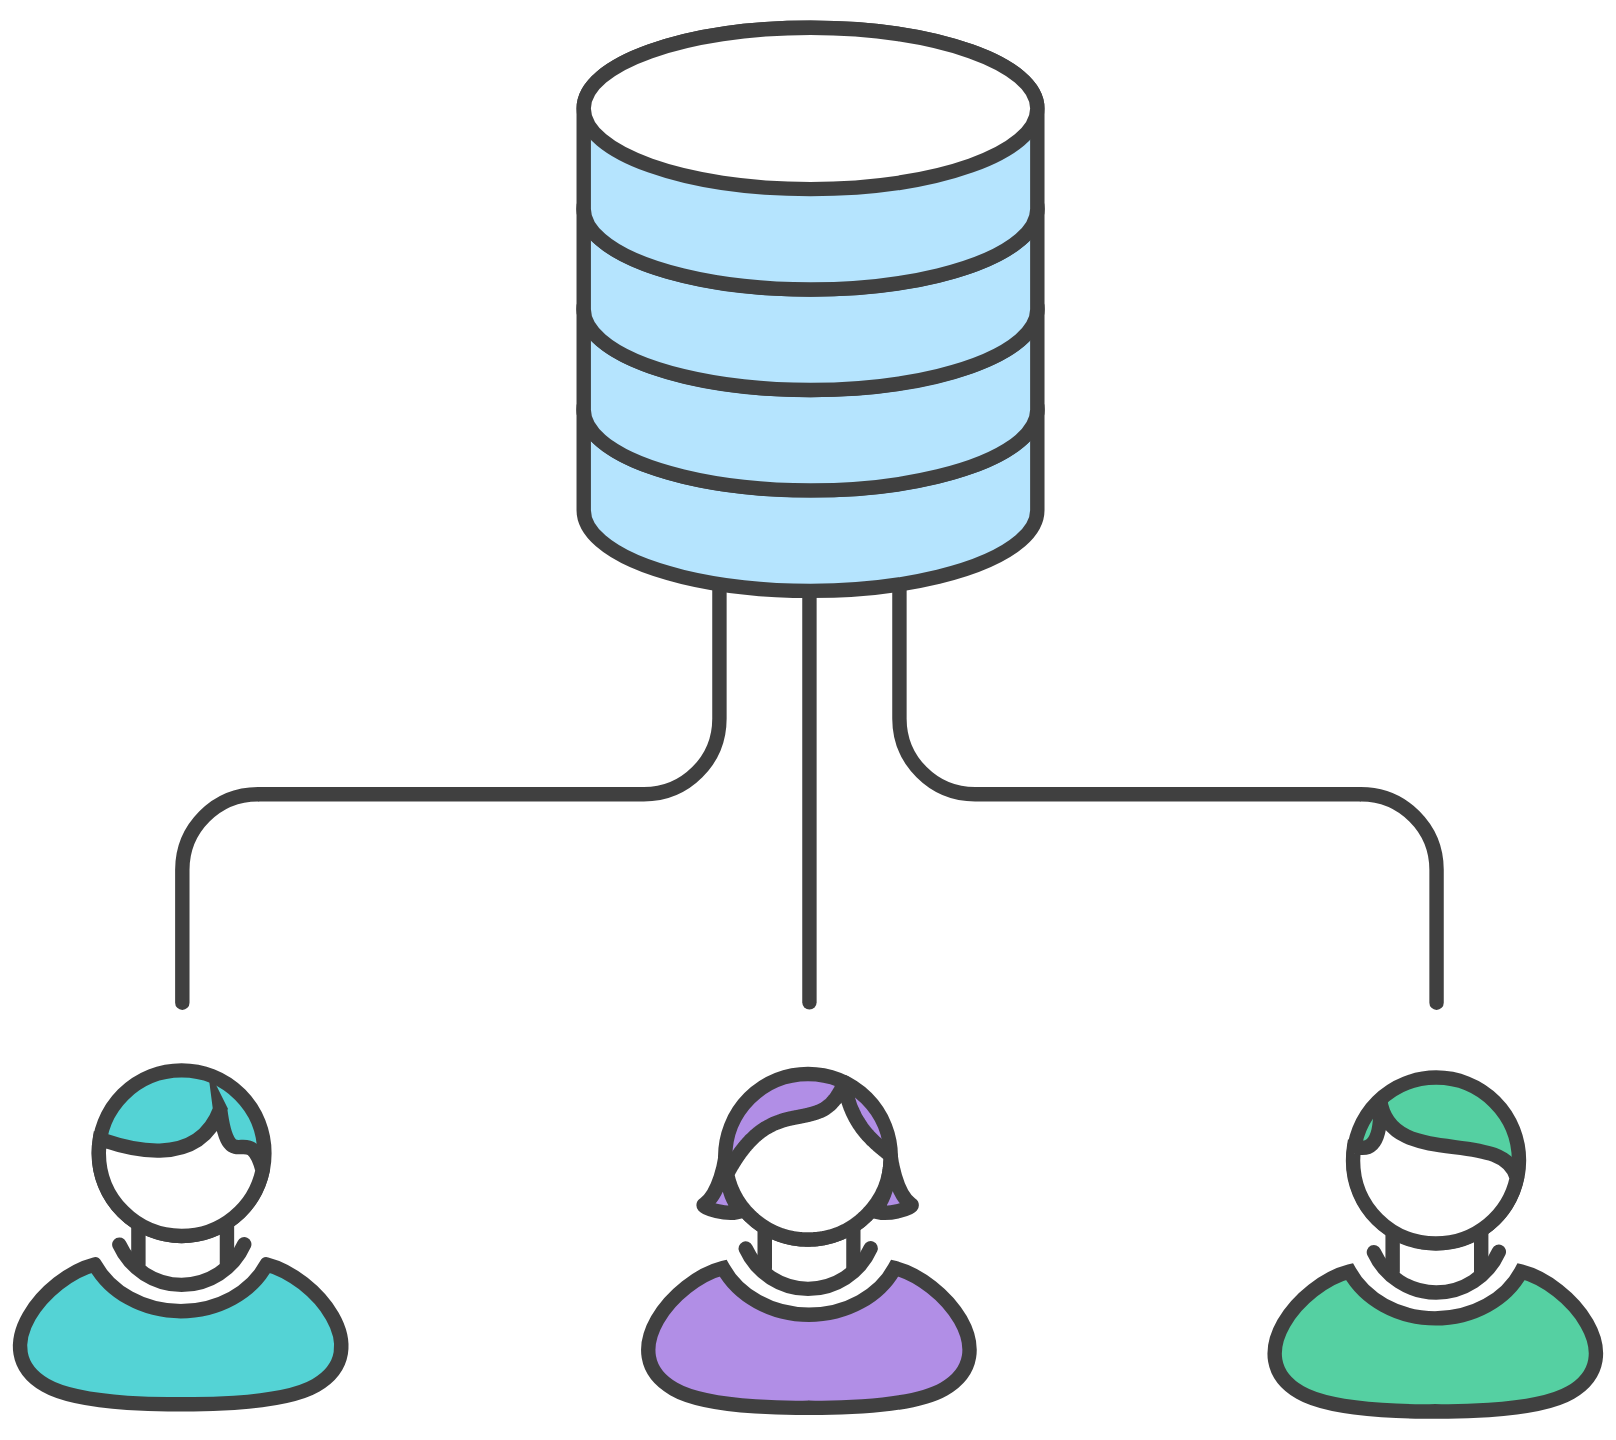
\includegraphics[scale=.15]{img/git-fluxo-centralizado.png}
\end{center}
}

\SliT{Fluxo de trabalho centralizado}{
\begin{itemize}

    \iOn{Não requer nenhum outro \textit{branch} além da \texttt{master}}

    \iOn{\textbf{O mais simples dos fluxos de trabalho}}

    \iOn{Como funciona:}

    \begin{itemize}
    
        \iTw{\texttt{clone} do repositório central}

        \iTw{Em cópias locais são feitas edições dos arquivos e confirmação das
            mudanças (\texttt{git add \& git commit})}

        \iTw{Fazer \texttt{push} da \textit{branch} \texttt{master} local para
            o repositório remoto;}
    
    \end{itemize}

\end{itemize}
}

\begin{SliTC}{Fluxo de trabalho centralizado}
Exemplo:
\begin{CodeD}{bash}
$ git clone <algum repositorio>
# Edição de arquivos;
$ git add <arquivos modificados>
$ git commit -m "descrição rápida de modificações"
$ git push origin master
\end{CodeD}
\end{SliTC}


\SliT{Fluxo de trabalho centralizado}{
\begin{itemize}

    \iOn{Conflitos:}

\end{itemize}

\begin{center}
    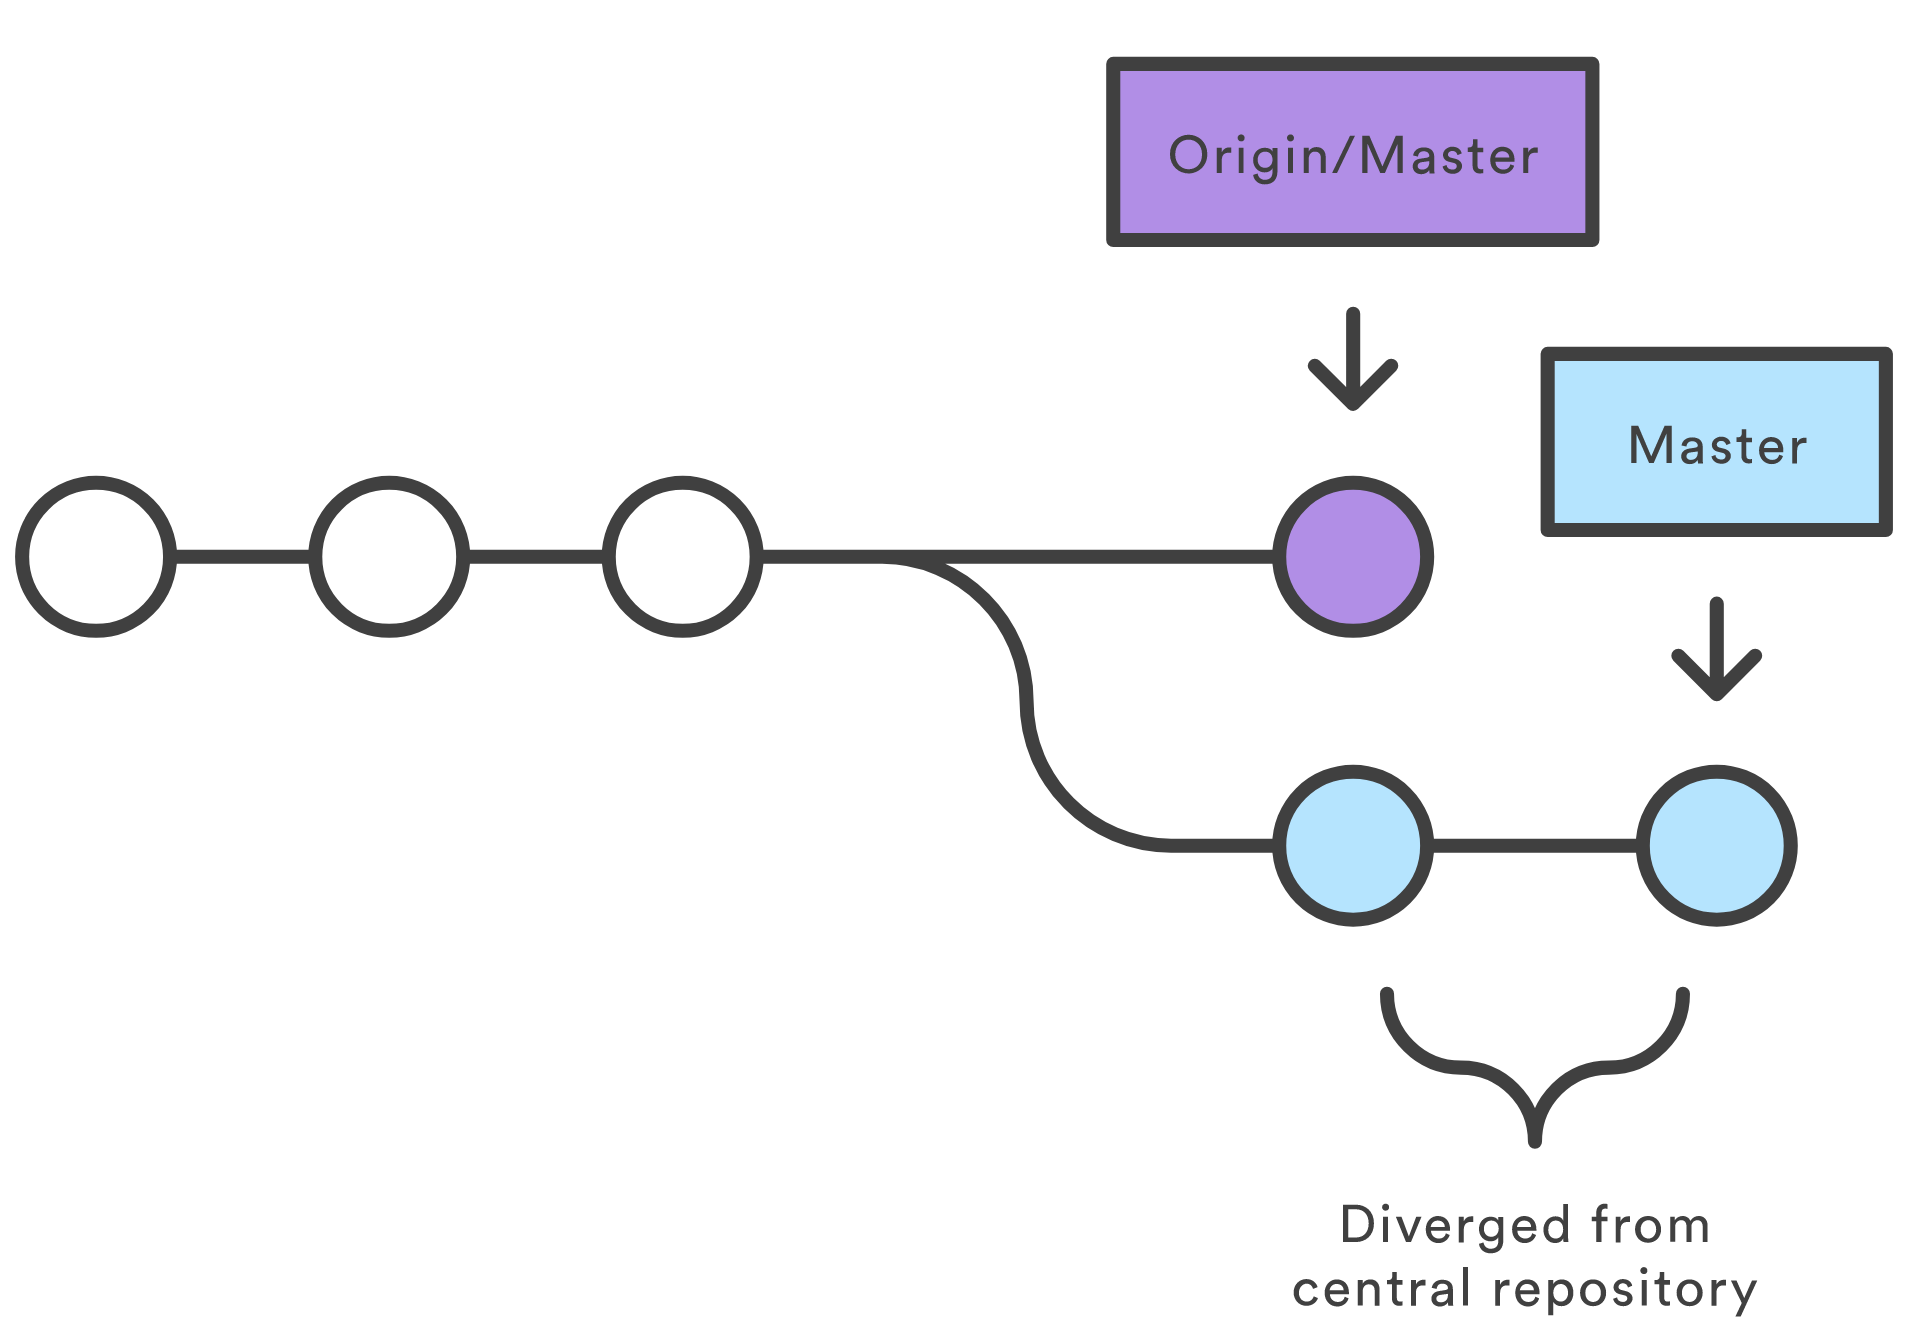
\includegraphics[scale=.2]{img/git-fluxo-centralizado-conflito1.png}
\end{center}
}


\SliT{Fluxo de trabalho centralizado}{
\begin{itemize}

    \iOn{Resolvendo conflitos (exemplo):}

    \begin{itemize}
    
        \iTw{John trabalha nas suas mudanças}
    
    \end{itemize}

\end{itemize}

\begin{center}
    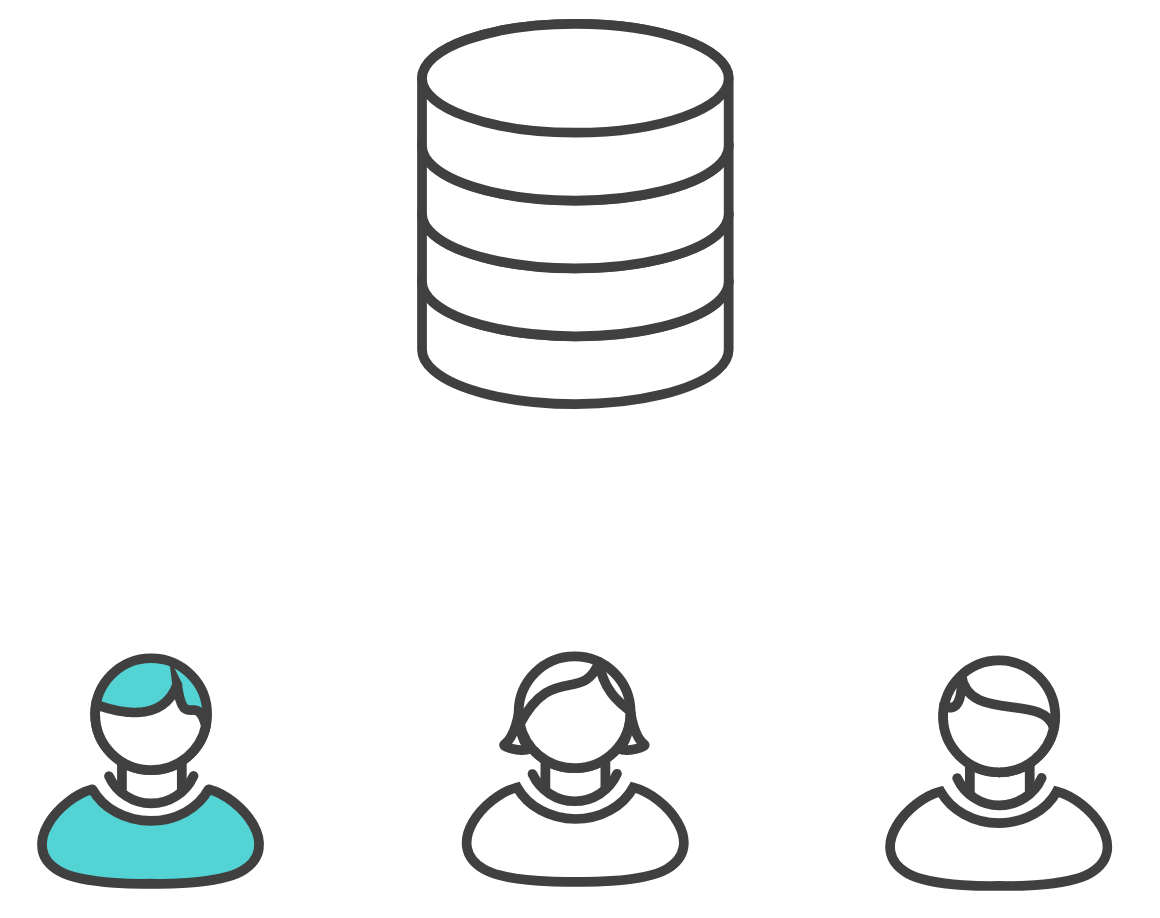
\includegraphics[scale=.2]{img/git-fluxo-centralizado-conflito2.png}
\end{center}

}


\SliT{Fluxo de trabalho centralizado}{
\begin{itemize}

    \iOn{Resolvendo conflitos (exemplo):}

    \begin{itemize}
    
        \iTw{Mary trabalha nas suas mudanças}
    
    \end{itemize}

\end{itemize}

\begin{center}
    
\includegraphics[scale=.2]{img/git-fluxo-centralizado-conflito3.png}
\end{center}

}


\begin{SliTC}{Fluxo de trabalho centralizado}
\begin{itemize}

    \iOn{Resolvendo conflitos (exemplo):}

    \begin{itemize}
    
        \iTw{John publica suas mudanças}
    
    \end{itemize}

\end{itemize}

\begin{center}
    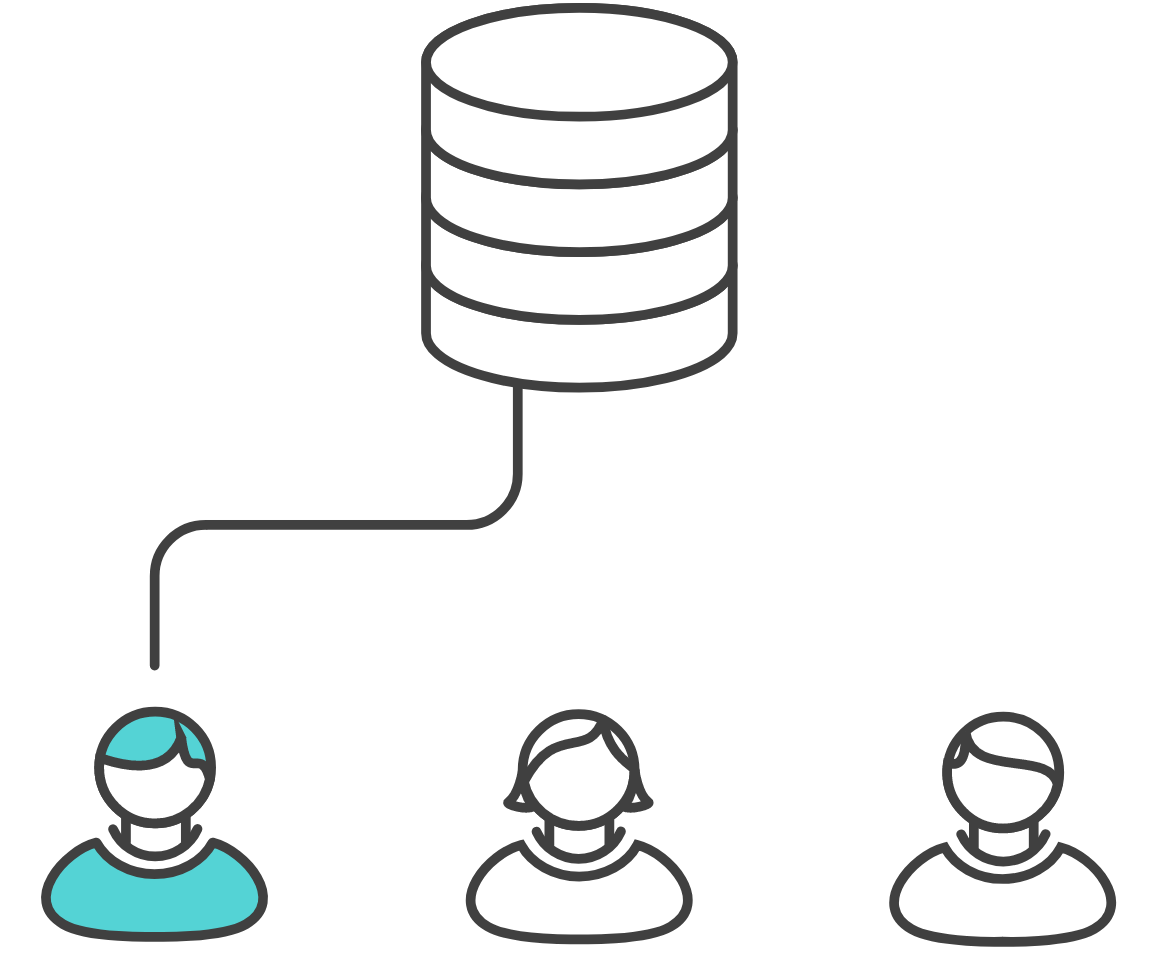
\includegraphics[scale=.2]{img/git-fluxo-centralizado-conflito4.png}
\end{center}

\begin{CodeD}{bash}
$ git push origin master
\end{CodeD}

\end{SliTC}


\begin{SliTC}{Fluxo de trabalho centralizado}
\begin{itemize}

    \iOn{Resolvendo conflitos (exemplo):}

    \begin{itemize}
    
        \iTw{Mary tenta publicar suas mudanças}
    
    \end{itemize}

\end{itemize}

\begin{center}
    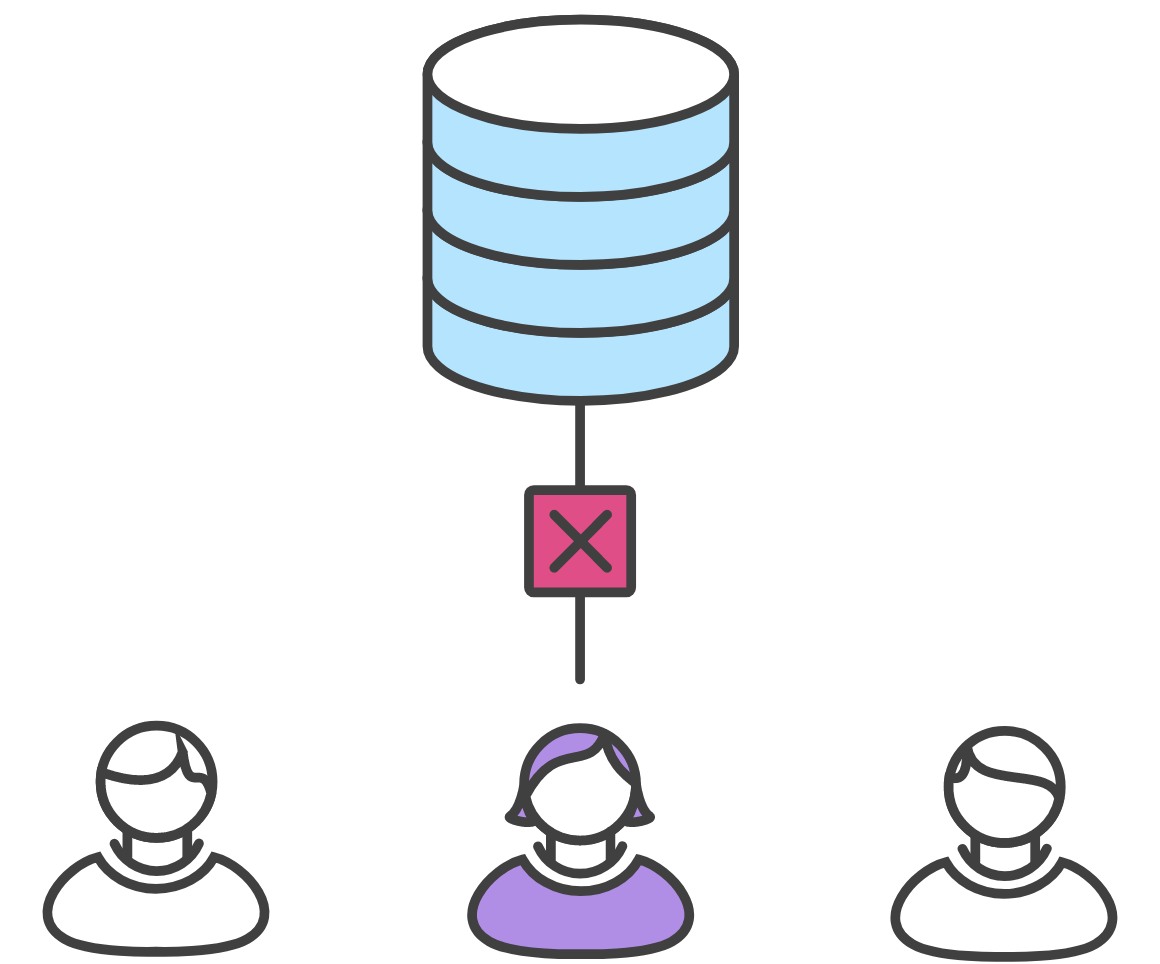
\includegraphics[scale=.2]{img/git-fluxo-centralizado-conflito5.png}
\end{center}

\begin{CodeD}{bash}
$ git push origin master
\end{CodeD}

\end{SliTC}


\begin{SliTC}{Fluxo de trabalho centralizado}
\begin{itemize}

    \iOn{Resolvendo conflitos (exemplo):}

    \begin{itemize}
    
        \iTw{Mary tenta publicar suas mudanças}
    
    \end{itemize}

\end{itemize}

\begin{CodeD}{bash}
 ! [rejected]        master -> master (fetch first)
error: failed to push some refs to '/Users/rocknroll/github/meu-repositorio'
hint: Updates were rejected because the remote contains work that you do
hint: not have locally. This is usually caused by another repository pushing
hint: to the same ref. You may want to first integrate the remote changes
hint: (e.g., 'git pull ...') before pushing again.
hint: See the 'Note about fast-forwards' in 'git push --help' for details.
\end{CodeD}

\end{SliTC}



\begin{SliTC}{Fluxo de trabalho centralizado}
\begin{itemize}

    \iOn{Resolvendo conflitos (exemplo):}

    \begin{itemize}
    
        \iTw{Mary faz o \texttt{rebase} de suas mudanças}
    
    \end{itemize}

\end{itemize}

\begin{center}
    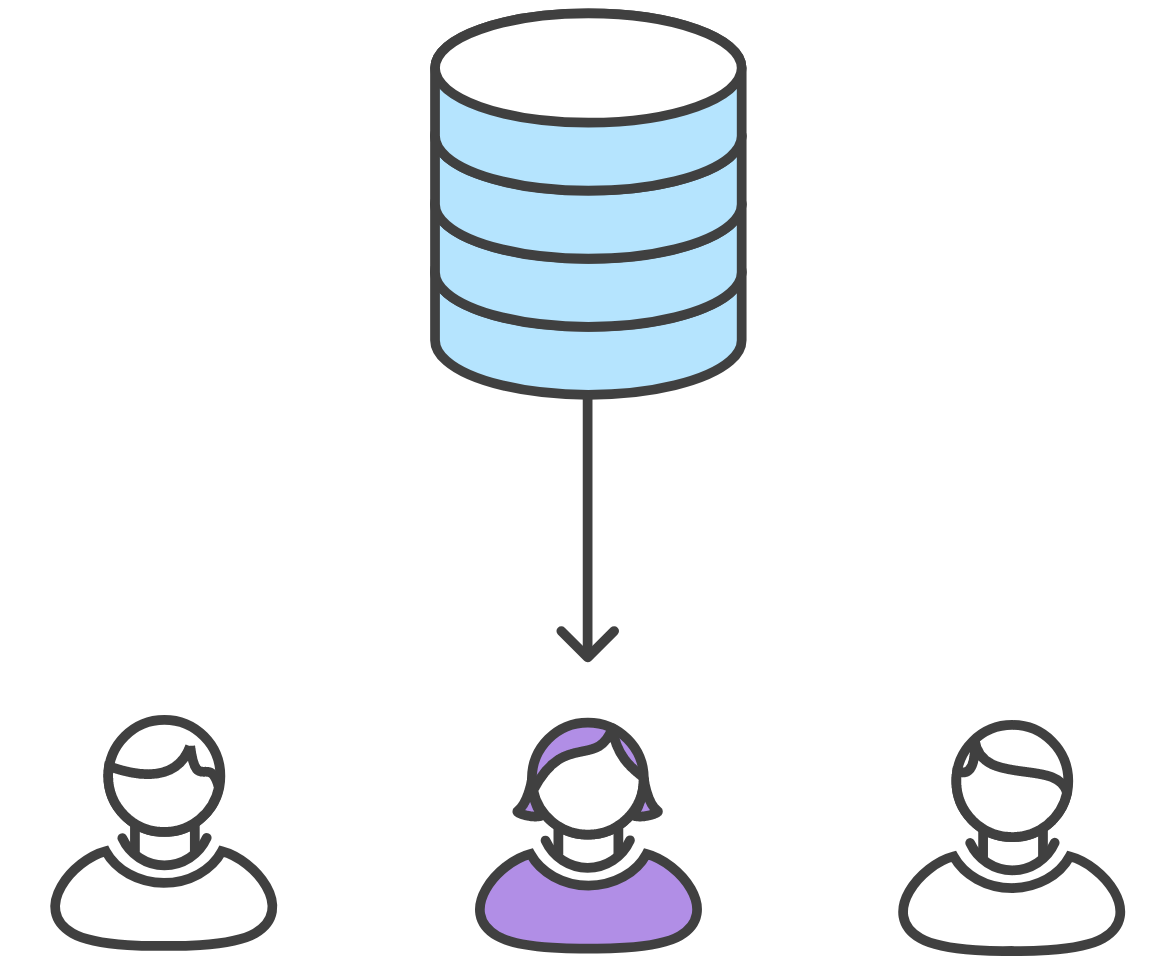
\includegraphics[scale=.2]{img/git-fluxo-centralizado-conflito6.png}
\end{center}

\begin{CodeD}{bash}
$ git pull --rebase origin master
\end{CodeD}

\end{SliTC}


\begin{SliTC}{Fluxo de trabalho centralizado}
\begin{itemize}

    \iOn{Resolvendo conflitos (exemplo):}

    \begin{itemize}
    
        \iTw{\texttt{--rebase} diz ao Git para mover todos os commits de Mary
            para a ponta da ramificação mestre}
    
    \end{itemize}

\end{itemize}

\begin{center}
    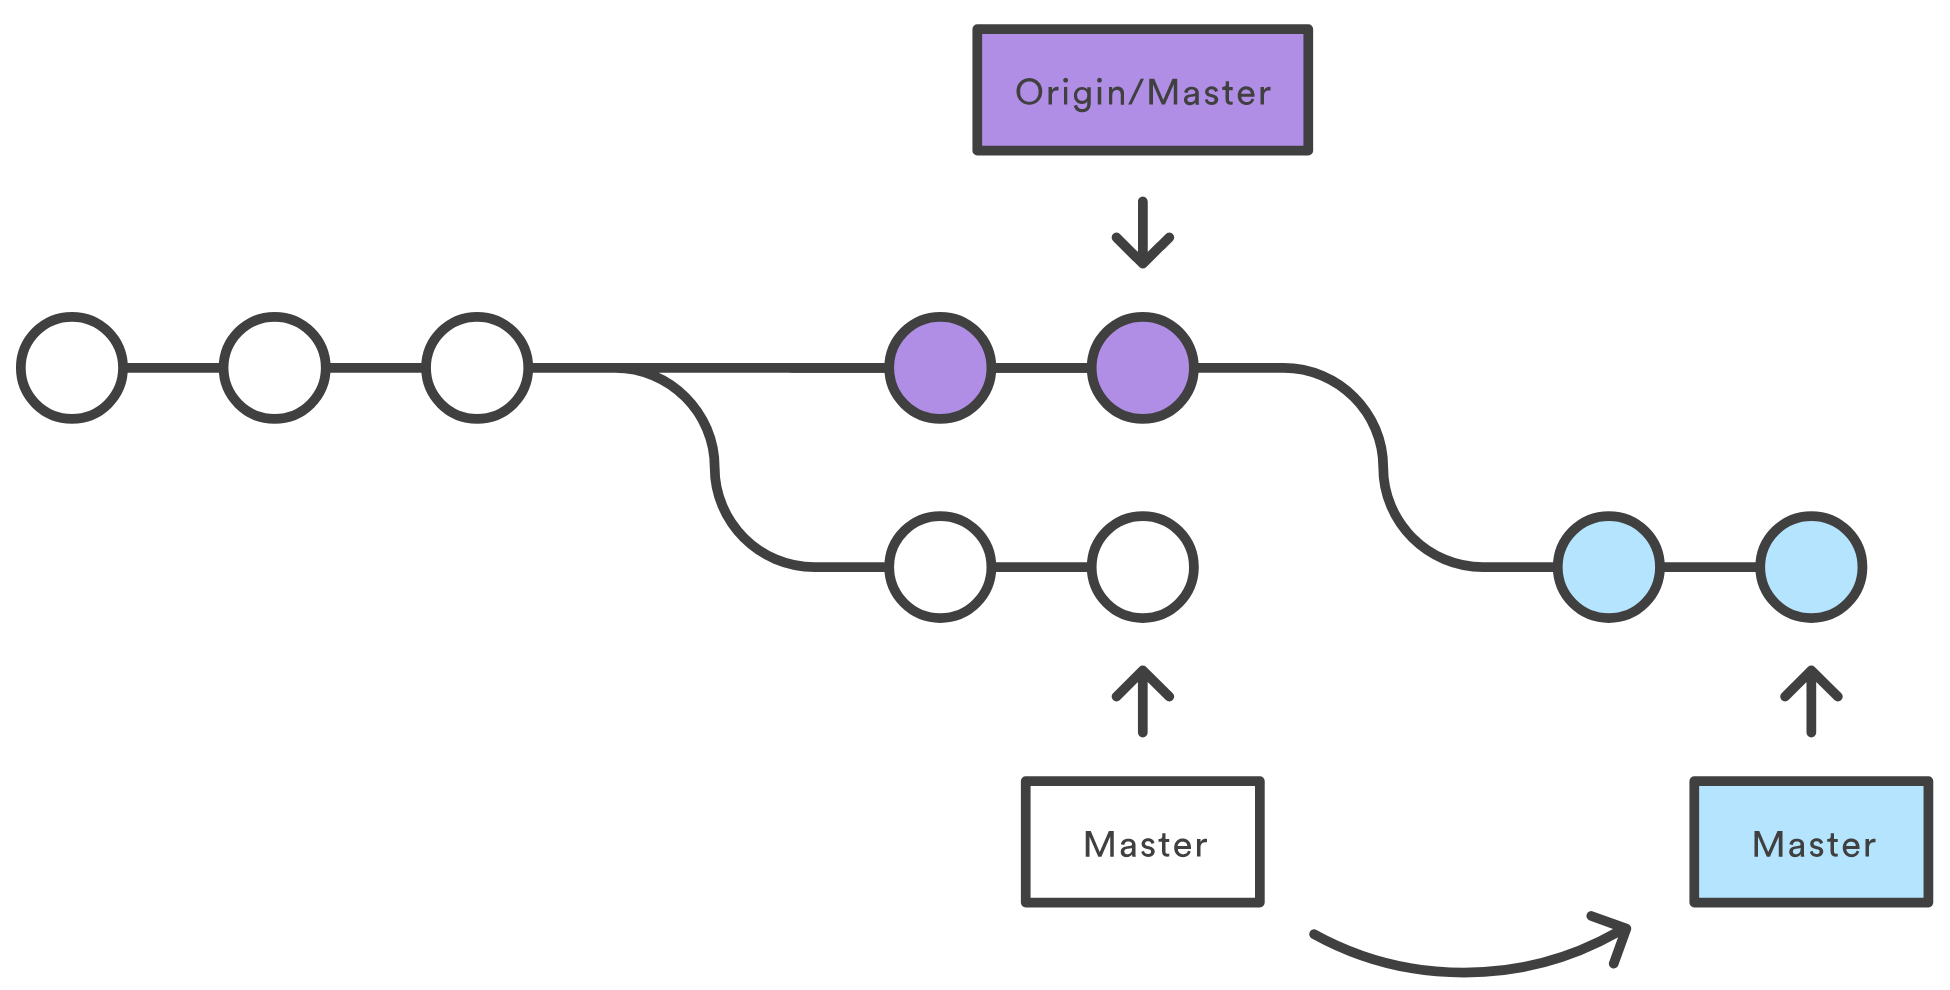
\includegraphics[scale=.25]{img/git-fluxo-centralizado-conflito7.png}
\end{center}

\end{SliTC}


\begin{SliTC}{Fluxo de trabalho centralizado}
\begin{itemize}

    \iOn{Resolvendo conflitos (exemplo):}

    \begin{itemize}
    
        \iTw{Se Mary e John estiverem trabalhando em recursos não relacionados,
            é improvável que o rebase gere conflitos. }

        \iTw{Em caso de recursos relacionados, o Git vai pausar o rebase na
            confirmação atual e enviar a seguinte mensagem, juntamente com
            algumas instruções relevantes:}
    
    \end{itemize}

\end{itemize}

\begin{CodeD}{bash}
CONFLICT (content): Merge conflict in <file>
Resolve all conflicts manually, mark them as resolved with
"git add/rm <conflicted_files>", then run "git rebase --continue".
\end{CodeD}

\end{SliTC}


\begin{SliTC}{Fluxo de trabalho centralizado}
\begin{itemize}

    \iOn{Resolvendo conflitos (exemplo):}

    \begin{itemize}
    
        \iTw{Verificando o status no repositório de Mary}

    \end{itemize}

\end{itemize}

\begin{CodeD}{bash}
$ git status
Unmerged paths:
  (use "git restore --staged <file>..." to unstage)
  (use "git add <file>..." to mark resolution)
  both modified:   <file>
\end{CodeD}

\end{SliTC}


\begin{SliTC}{Fluxo de trabalho centralizado}
\begin{itemize}

    \iOn{Resolvendo conflitos (exemplo):}

    \begin{itemize}
    
        \iTw{Verificando o conflito no repositório de Mary}

    \end{itemize}

\end{itemize}

\begin{CodeD}{bash}
<<<<<<< HEAD
<Local File Content>
=======
<Remote File Content>
>>>>>>> Remote Repo Commit Message
<Common ContentL>
\end{CodeD}

\end{SliTC}


\begin{SliTC}{Fluxo de trabalho centralizado}
\begin{itemize}

    \iOn{Resolvendo conflitos (exemplo):}

    \begin{itemize}
    
        \iTw{Continuando a operação de \texttt{rebase}}

    \end{itemize}

\end{itemize}

\begin{CodeD}{bash}
$ git rebase --continue
\end{CodeD}

\end{SliTC}


\begin{SliTC}{Fluxo de trabalho centralizado}
\begin{itemize}

    \iOn{Resolvendo conflitos (exemplo):}

    \begin{itemize}
    
        \iTw{Resultado do \texttt{rebase} no histórico de commits}
        \iTw{Discussão \textit{Rebase} vs \textit{Merge}}

    \end{itemize}

\end{itemize}

\begin{center}
    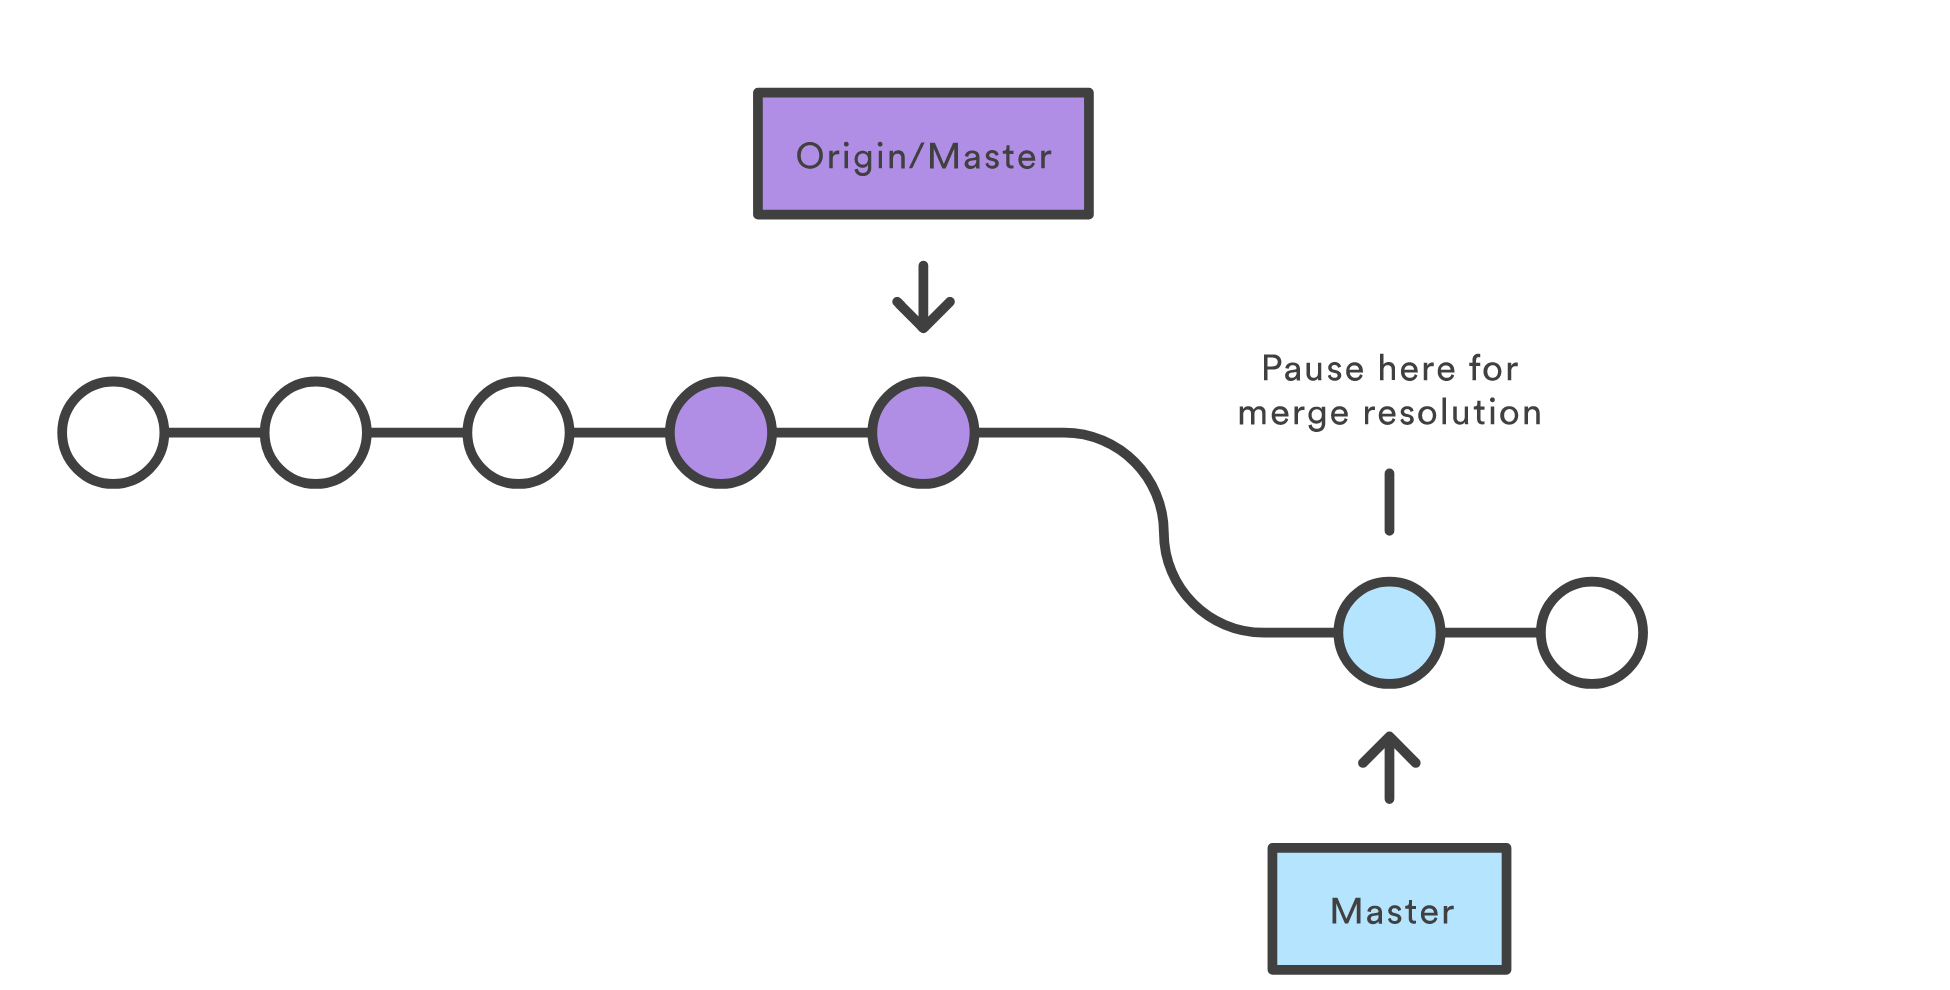
\includegraphics[scale=.25]{img/git-fluxo-centralizado-conflito8.png}
\end{center}

\end{SliTC}

\SliSubTit{Feature Branch Workflow}{}


\SliT{Fluxo de trabalho de Branch por Feature}{
\begin{itemize}

    \iOn{Focado no modelo de branch por nova funcionalidade}

    \iOn{Desenvolvimento de \textit{features} deve ocorrer em um branch
        dedicado}

    \iOn{Facilita o trabalho em uma \textit{feature} específica sem interromper
        a principal base de código}

    \iOn{\textbf{\textit{branch} principal nunca vai conter um código
        quebrado}}

    \iOn{\textit{pull requests} para iniciar discussões em torno de um
        \textit{branch}}

    \iOn{Oportunidade de aprovar uma funcionalidade antes de ser integrado ao
        projeto oficial}

\end{itemize}
}

\SliT{Fluxo de trabalho de Branch por Feature}{
\begin{itemize}

    \iOn{O \textit{branch} principal representa o histórico oficial do projeto}

    \iOn{Os branches dos recursos devem ter nomes descritivos:}

    \begin{itemize}
    
        \iTw{\texttt{issue-\#1061}, se relacionada a uma \textit{issue}
            específica}

        \iTw{\texttt{carregamento-de-dados}, se o nome reflete uma
            \textit{feature} específica}
    
    \end{itemize}

    \iOn{Dar um objetivo claro e bastante focado a cada \textit{branch}}

    \iOn{Os branches de \textit{features} devem ser enviados para o repositório
        remoto}

\end{itemize}
}


\begin{SliTC}{Fluxo de trabalho de Branch por Feature}
\begin{itemize}

    \iOn{Passo-a-passo}

    \begin{itemize}
    
        \iTw{Certificar-se que a branch \texttt{master} está atualizado com a
            cópia remota}
    
        \iTw{\texttt{git reset --hard origin/master} vai limpar todas as
            modificações locais feitas na branch \texttt{master}}

    \end{itemize}

\end{itemize}


\begin{CodeD}{bash}
$ git checkout master
$ git fetch origin
$ git reset --hard origin/master
\end{CodeD}

\end{SliTC}


\begin{SliTC}{Fluxo de trabalho de Branch por Feature}
\begin{itemize}

    \iOn{Passo-a-passo}

    \begin{itemize}
    
        \iTw{Criar nova branch baseada na \texttt{master} para a nova
            \textit{feature}}

    \end{itemize}

\end{itemize}


\begin{CodeD}{bash}
$ git checkout -b nova-feature
\end{CodeD}

\end{SliTC}


\begin{SliTC}{Fluxo de trabalho de Branch por Feature}
\begin{itemize}

    \iOn{Passo-a-passo}

    \begin{itemize}
    
        \iTw{Escrever modificações, adicioná-las e realizar o \textit{commit}}

    \end{itemize}

\end{itemize}


\begin{CodeD}{bash}
$ git add <arquivo>
$ git commit -m "Mensagem de Commit"
\end{CodeD}

\end{SliTC}


\begin{SliTC}{Fluxo de trabalho de Branch por Feature}
\begin{itemize}

    \iOn{Passo-a-passo}

    \begin{itemize}
    
        \iTw{Enviar branch do recurso para repositório remoto}

    \end{itemize}

\end{itemize}


\begin{CodeD}{bash}
$ git push -u origin nova-feature
\end{CodeD}

\end{SliTC}


\SliT{Fluxo de trabalho de Branch por Feature}{
\begin{itemize}

    \iOn{Passo-a-passo}

    \begin{itemize}
    
        \iTw{Criando \textit{pull-request}}
    
    \end{itemize}

\end{itemize}
\begin{center}
    \begin{center}
        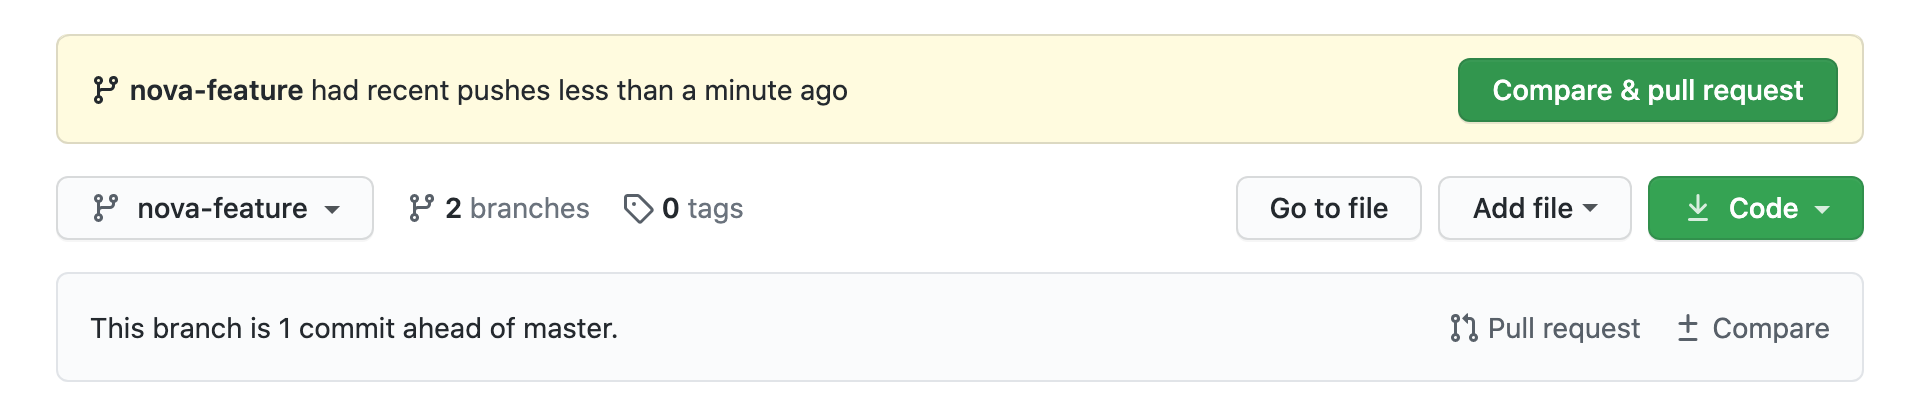
\includegraphics[scale=.4]{img/git-fluxo-feature-branch1.png}
    \end{center}
\end{center}

}


\SliT{Fluxo de trabalho de Branch por Feature}{
\begin{itemize}

    \iOn{Passo-a-passo}

    \begin{itemize}
    
        \iTw{Criando \textit{pull-request}}
    
    \end{itemize}

\end{itemize}
\begin{center}
    \begin{center}
        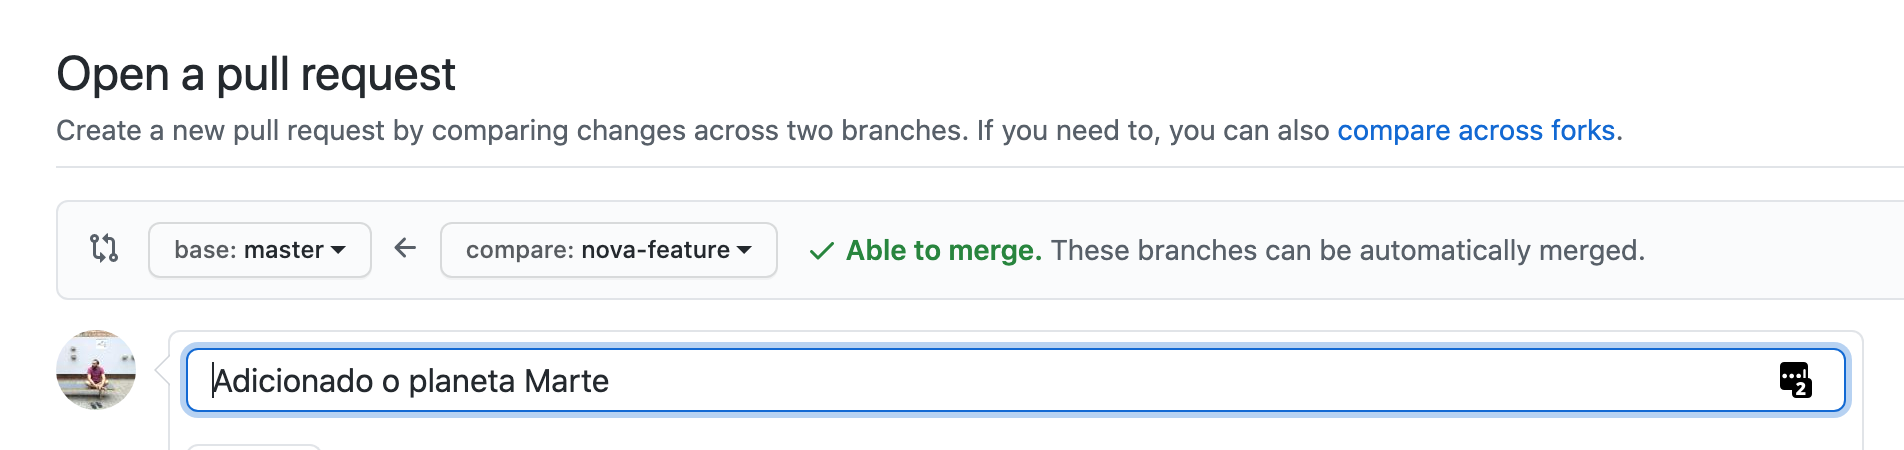
\includegraphics[scale=.4]{img/git-fluxo-feature-branch2.png}
    \end{center}
\end{center}

}


\SliT{Fluxo de trabalho de Branch por Feature}{
\begin{itemize}

    \iOn{Passo-a-passo}

    \begin{itemize}
    
        \iTw{Aceitando \textit{pull-request}}
    
    \end{itemize}

\end{itemize}
\begin{center}
    \begin{center}
        
\includegraphics[scale=.4]{img/git-fluxo-feature-branch3.png}
    \end{center}
\end{center}

}

\SliT{Fluxo de trabalho de Branch por Feature}{
\begin{itemize}

    \iOn{Caso a branch da nova \textit{feature} esteja atrás da
        \textit{master}}

\end{itemize}

\begin{center}
    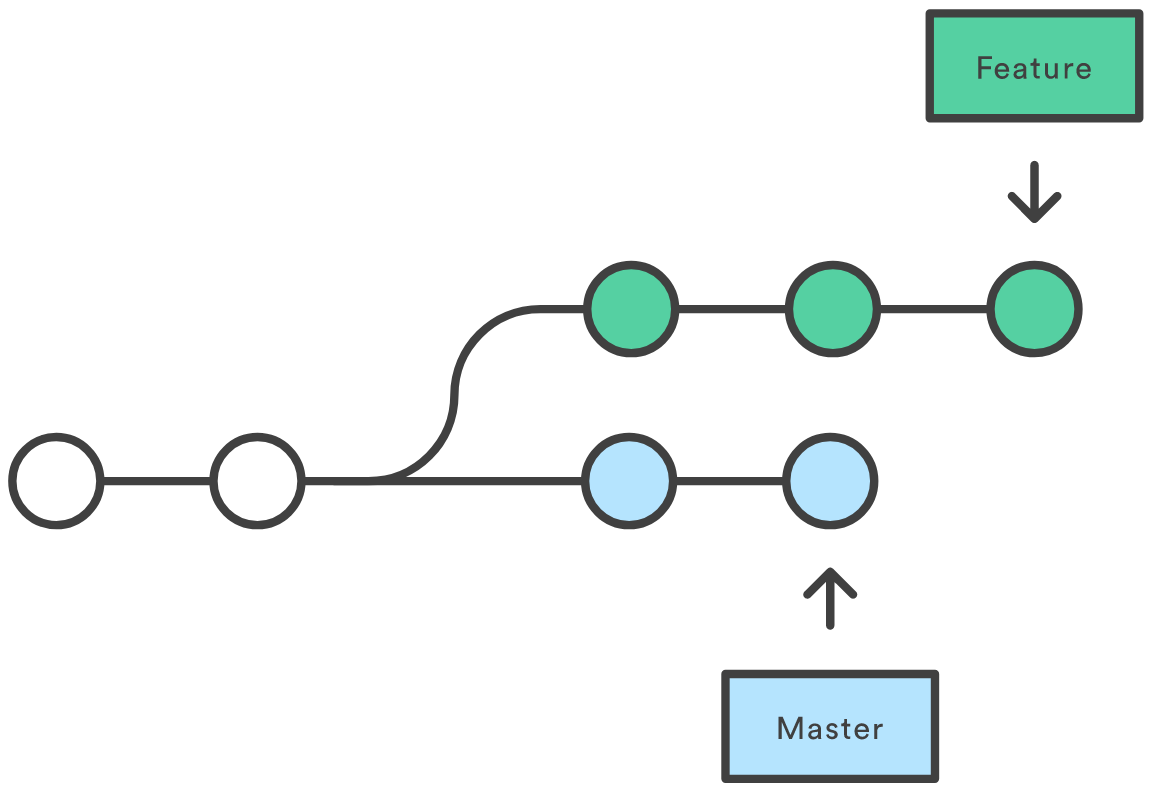
\includegraphics[scale=.35]{img/git-fluxo-feature-branch-rebase1.png}
\end{center}

}


\SliT{Fluxo de trabalho de Branch por Feature}{
\begin{itemize}

    \iOn{\texttt{rebase} para atualizar branch}

\end{itemize}

\begin{center}
    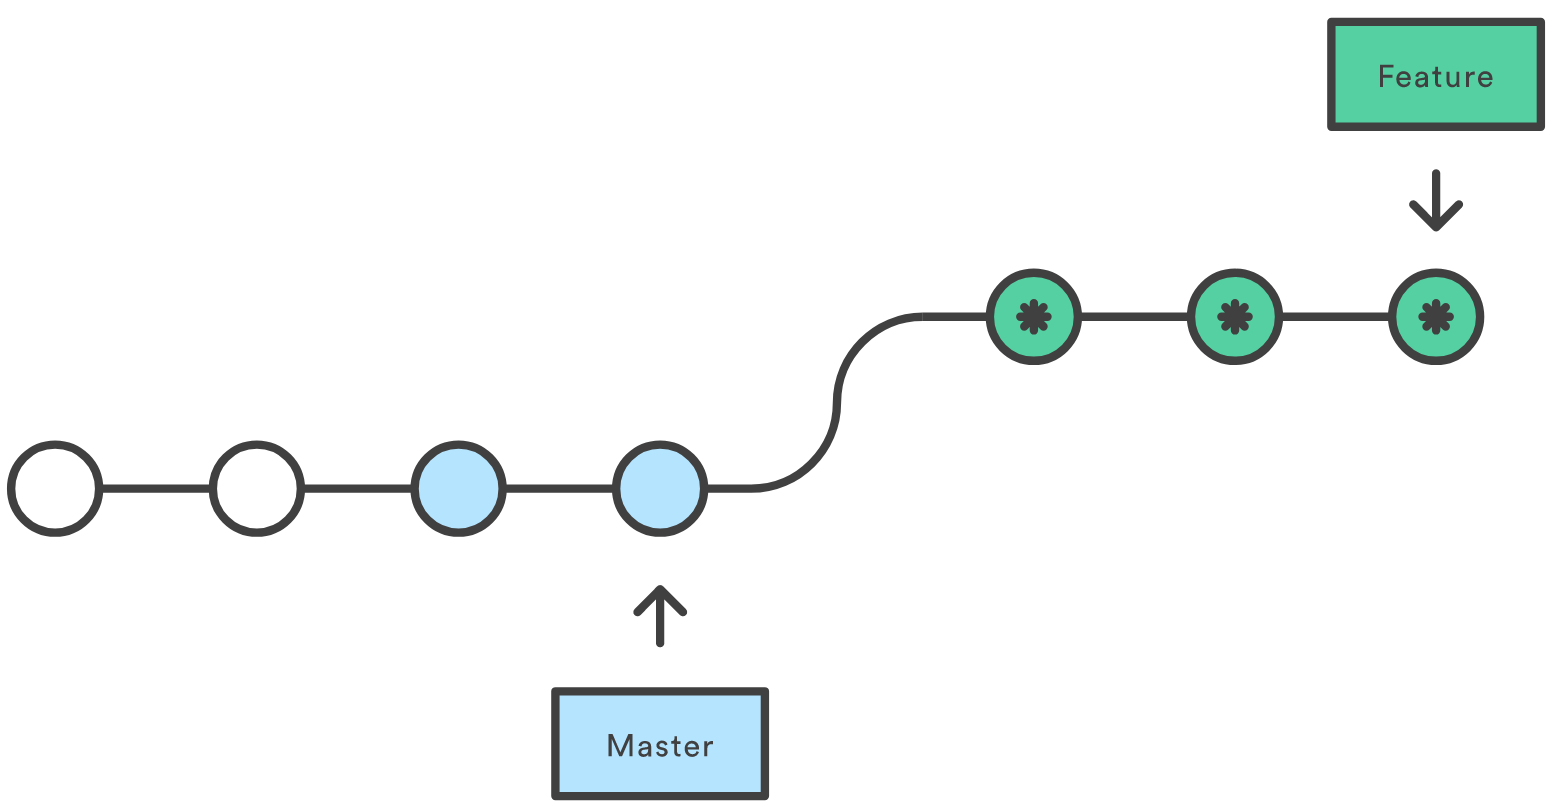
\includegraphics[scale=.35]{img/git-fluxo-feature-branch-rebase2.png}
\end{center}

}


\SliT{Fluxo de trabalho de Branch por Feature}{
\begin{itemize}

    \iOn{\textbf{A regra de ouro para o \texttt{rebase}}}

    \begin{itemize}
    
        \iTw{{\color{red}Nunca realizar rebase em branches públicas!}}
    
    \end{itemize}

\end{itemize}

\begin{center}
    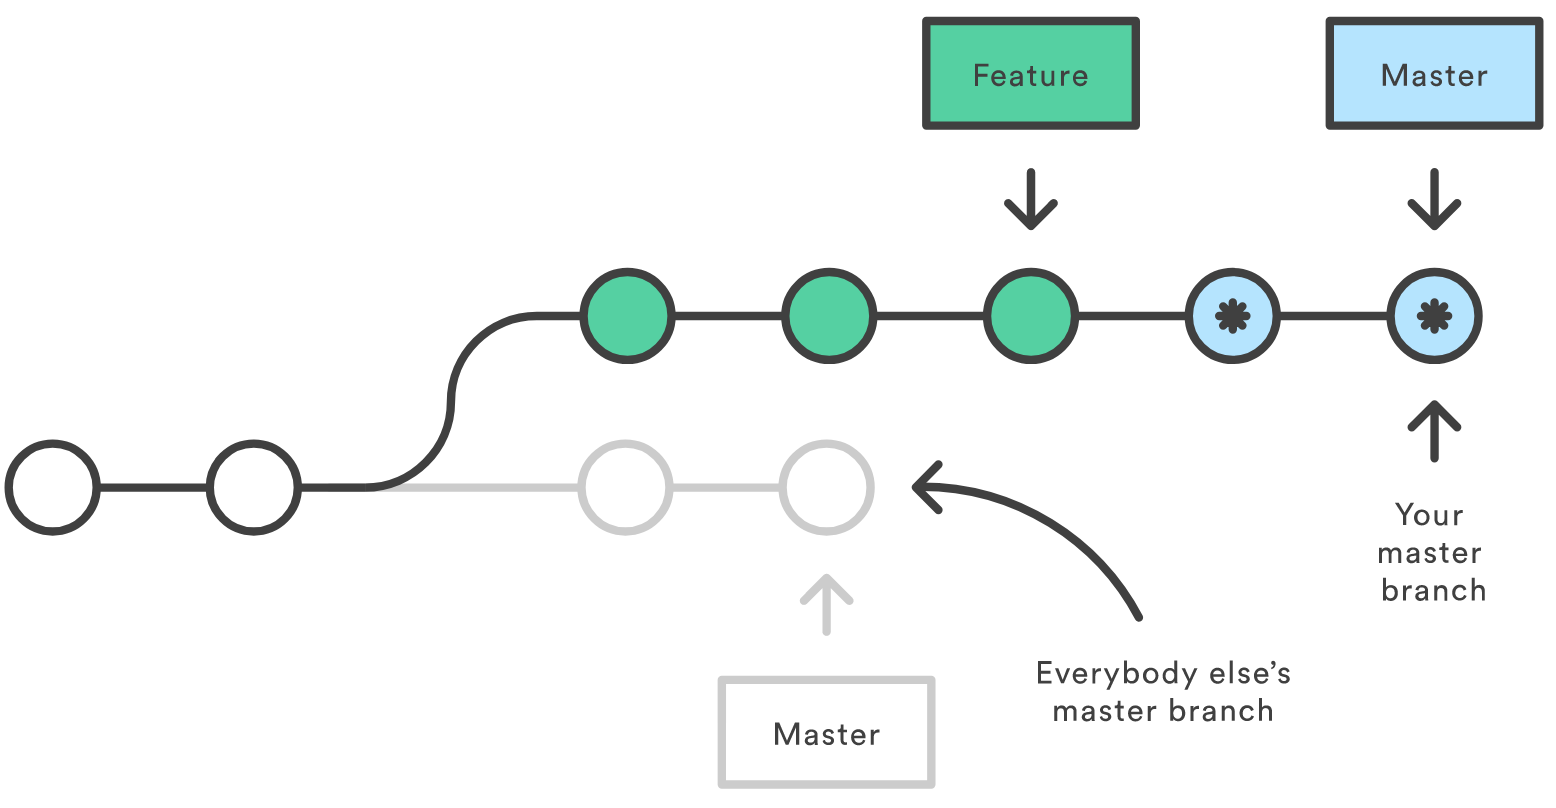
\includegraphics[scale=.35]{img/git-fluxo-feature-branch-rebase3.png}
\end{center}

}


\SliSubTit{Forking Workflow}{}

\SliT{Fluxo de trabalho baseado em Forks}{
\begin{itemize}

    \iOn{No Forking Workflow o usuário possui dois repositórios: um
        \textbf{privado (pessoal)} e um \textbf{publico (principal/central)}.}

    \iOn{Conceito de ``validação e aprovação''}

    \begin{itemize}
    
        \iTw{Focado na qualidade do projeto e no nível de abertura para
            contribuições;}

        \iTw{Colaboradores não precisam necessariamente de permissões para dar
            push no repositório oficial}

        \iTw{Submissão de \textit{Pull Requests} para o repositório principal}

        \iTw{Após a revisão, correções são feitas no fork privado e agregando
            alterações ao \textit{pull request}}
    
    \end{itemize}

\end{itemize}
}


\SliT{Fluxo de trabalho baseado em Forks}{
\begin{itemize}

    \iOn{Como funciona?}

    \begin{itemize}
    
        \iTw{Criando um fork no github.}
    
    \end{itemize}

\end{itemize}

\begin{center}
    
\includegraphics[scale=.5]{img/git-fluxo-fork1.png}
\end{center}

}



\begin{SliTC}{Fluxo de trabalho baseado em Forks}

\begin{itemize}

    \iOn{Como funciona?}

    \begin{itemize}
    
        \iTw{Clonar seu fork}
    
    \end{itemize}

\end{itemize}


    \begin{CodeD}{bash}
$ git clone <repositorio do seu fork>
    \end{CodeD}
\end{SliTC}


\begin{SliTC}{Fluxo de trabalho baseado em Forks}

\begin{itemize}

    \iOn{Como funciona?}

    \begin{itemize}
    
        \iTw{Adicionar novo repositório remoto (e.g., \texttt{upstream})}
    
    \end{itemize}

\end{itemize}


    \begin{CodeD}{bash}
$ git remote add upstream <repositorio de onde você realizou o fork>
    \end{CodeD}
\end{SliTC}


\begin{SliTC}{Fluxo de trabalho baseado em Forks}

\begin{itemize}

    \iOn{Como funciona?}

    \begin{itemize}
    
        \iTw{Criar branch para nova \textit{feature}}
    
    \end{itemize}

\end{itemize}


    \begin{CodeD}{bash}
$ git checkout -b nova-feature
# Edit some code
$ git commit -a -m "<Mensagem de Commit>"
    \end{CodeD}
\end{SliTC}


\begin{SliTC}{Fluxo de trabalho baseado em Forks}

\begin{itemize}

    \iOn{Como funciona?}

    \begin{itemize}
    
        \iTw{Enviar branch para o seu repositório privado remoto}
    
    \end{itemize}

\end{itemize}


    \begin{CodeD}{bash}
$ git push origin nova-feature
    \end{CodeD}
\end{SliTC}


\SliT{Fluxo de trabalho baseado em Forks}{
\begin{itemize}

    \iOn{Como funciona?}

    \begin{itemize}
    
        \iTw{Criando um pull request}
    
    \end{itemize}

\end{itemize}

\begin{center}
    
\includegraphics[scale=.4]{img/git-fluxo-fork2.png}
\end{center}

}


\SliT{Fluxo de trabalho baseado em Forks}{
\begin{itemize}

    \iOn{Como funciona?}

    \begin{itemize}
    
        \iTw{Aprovando um pull request}
    
    \end{itemize}

\end{itemize}

\begin{center}
    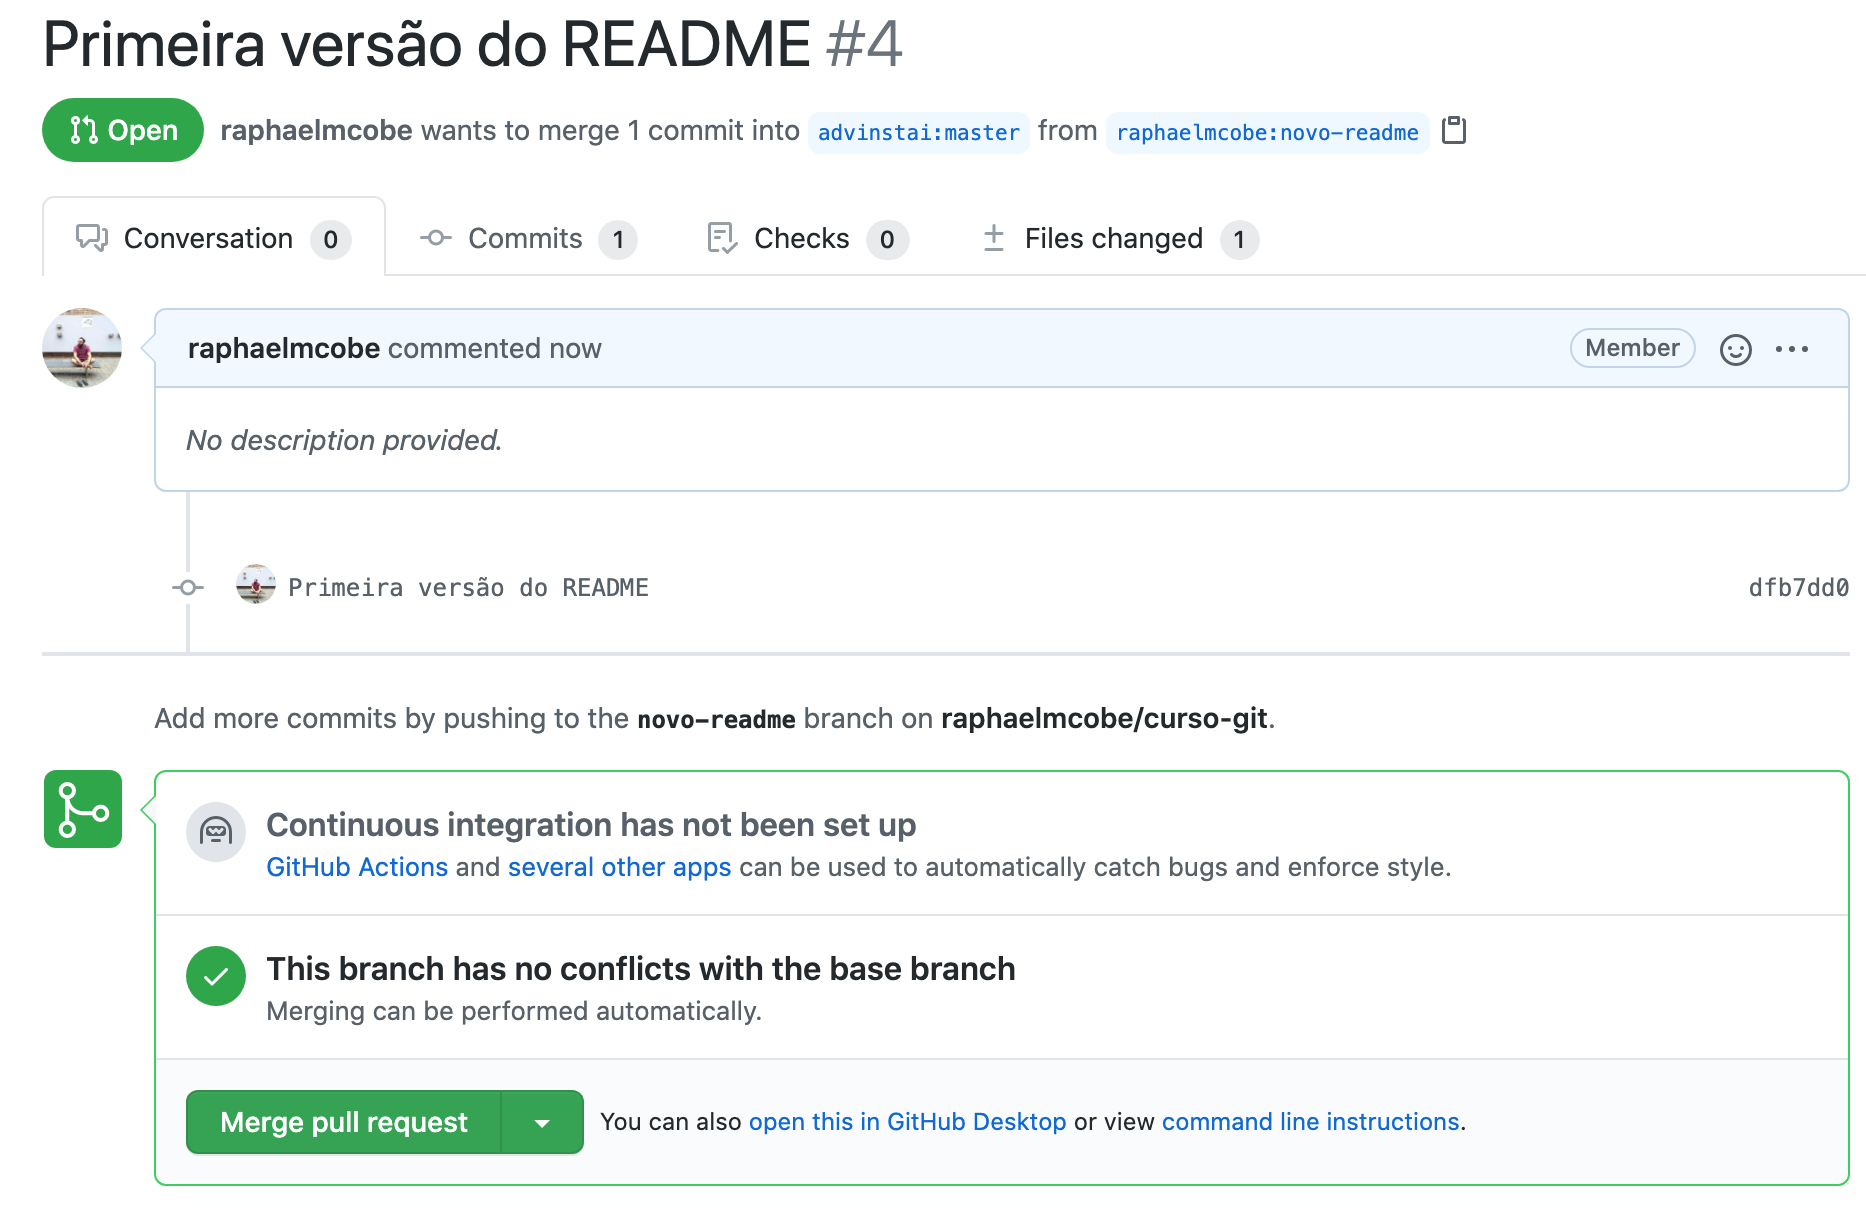
\includegraphics[scale=.25]{img/git-fluxo-fork3.png}
\end{center}

}


\begin{SliTC}{Fluxo de trabalho baseado em Forks}

\begin{itemize}

    \iOn{Como funciona?}

    \begin{itemize}
    
        \iTw{Atualizando branch com novas alterações enquanto você trabalha em
            sua funcionalidade}
    
    \end{itemize}

\end{itemize}


    \begin{CodeD}{bash}
$ git fetch upstream
$ git rebase upstream/master 
    \end{CodeD}
\end{SliTC}


\SliT{Considerações Finais}{

\begin{center}
    
\includegraphics[scale=.45]{img/luciano-ramalho-tweet.png}
\end{center}

\href{https://twitter.com/ramalhoorg}{@ramalhoorg}
}


\end{document}
